\documentclass[aspectratio=169]{beamer}
\useoutertheme[progressbar=frametitle]{metropolis}
\useinnertheme{metropolis}
\definecolor{nabgray}{rgb}{0.6,0.59,0.61}
\usecolortheme[named=nabgray]{structure}
\usepackage{tikz}
\usepackage{hyperref}
\usetikzlibrary{mindmap,backgrounds}
\usepackage[utf8]{inputenc}
\usepackage[spanish]{babel}
\usepackage{fontspec}
\setmonofont{JetBrains Mono}
\setmainfont{Roboto}
\setsansfont{Roboto}

\usepackage{smartdiagram}
\usepackage{qtree}
\usepackage{verbatim}
\usepackage{svg}
\usepackage{graphicx}
\usepackage{color}
\definecolor{lightgray}{rgb}{0.95, 0.95, 0.95}
\definecolor{darkgray}{rgb}{0.4, 0.4, 0.4}
\definecolor{ocherCode}{rgb}{1, 0.5, 0} % #FF7F00 -> rgb(239, 169, 0)
\definecolor{blueCode}{rgb}{0, 0, 0.93} % #0000EE -> rgb(0, 0, 238)
\definecolor{greenCode}{rgb}{0, 0.6, 0} % #009900 -> rgb(0, 153, 0) 

\usepackage{upquote}
\usepackage{listings}
\lstset{language=java,
    otherkeywords={var,record},
	% Basic design
	backgroundcolor=\color{lightgray},
	basicstyle={\small\ttfamily},   
	frame=l,
	keywordstyle=\footnotesize\color{blue},
	escapeinside={<@}{@>},
	breaklines=true,
	% Line numbers
	xleftmargin={0.75cm},
	numbers=left,
	stepnumber=1,
	firstnumber=1,
	numberfirstline=true
	% Code design
	identifierstyle=\color{black},
	keywordstyle=\color{ocherCode}\bfseries,
	ndkeywordstyle=\color{greenCode}\bfseries,
	stringstyle=\color{ocherCode}\ttfamily,
	commentstyle=\color{darkgray}\ttfamily,
	tabsize=2,
	showtabs=true,
	showspaces=false,
	showstringspaces=false,
	extendedchars=true,
	breaklines=true
}

\lstdefinelanguage{bash}{
    basicstyle=\ttfamily,
    showstringspaces=false,
    commentstyle=\color{red},
    keywordstyle=\color{blue},
    numbers=right,
    xleftmargin={0.25cm}
}

\usebackgroundtemplate
{
	
\includegraphics[width=\paperwidth]{Images/fondo}%
}


\title{Aprendizaje en tiempos de crisis}
\author{Víctor Orozco - @tuxtor}
\institute{Academik}
\date{\today}

\begin{document}

{
    \usebackgroundtemplate{
\includegraphics[width=\paperwidth]{Images/portada}}
    \setbeamercolor{frametitle}{fg=red}
    \usebeamercolor[fg]{normal text}
    \frame{\titlepage}
}

\begin{frame}[fragile]{¿Aprender en tiempos de crisis?}
	\begin{itemize}
		\item ¿Porque aprender nuevas habilidades?
		\item Modelos de aprendizaje en línea
		\item Herramientas de aprendizaje en línea
	\end{itemize}	
\end{frame}

\begin{frame}[fragile]{¿Porqué aprender nuevas habilidades?}
    \begin{center}
        
\includegraphics[width=0.6\linewidth]{Images/divertido}
    \end{center}	
\end{frame}

\begin{frame}[fragile]{¿Porqué aprender nuevas habilidades?}
    \begin{itemize}
        \item Porqué mi papá me obliga a estudiar
        \item Porqué me gustaría ser alguien en la vida
        \item Porqué me gusta el dinero
    \end{itemize}	
\end{frame}


\begin{frame}[fragile]{Capacitación}
    \begin{exampleblock}{Capacitación}
        En el estricto sentido formal, una capacitación es \textbf{una transferencia de conocimiento}, la cual puede ser para satisfacer una necesidad inmediata o futura.
        
        La clave es la inmediatez de la necesidad.
    \end{exampleblock}
\end{frame}

\begin{frame}[fragile]{Aprendizaje - Formas}
    \begin{itemize}
        \item Capacitación previa para adecuarse a un patrón (Certificación)
        \item Capacitación proactiva para mantener un nivel de capacidades (Mejora continua)
        \item Capacitación reactiva para transferencia inmediata de conocimientos (Necesidad, nuevo trabajo, despido inmediato)
    \end{itemize}
\end{frame}

\begin{frame}[fragile]{Capacitación previa}
    \begin{center}
        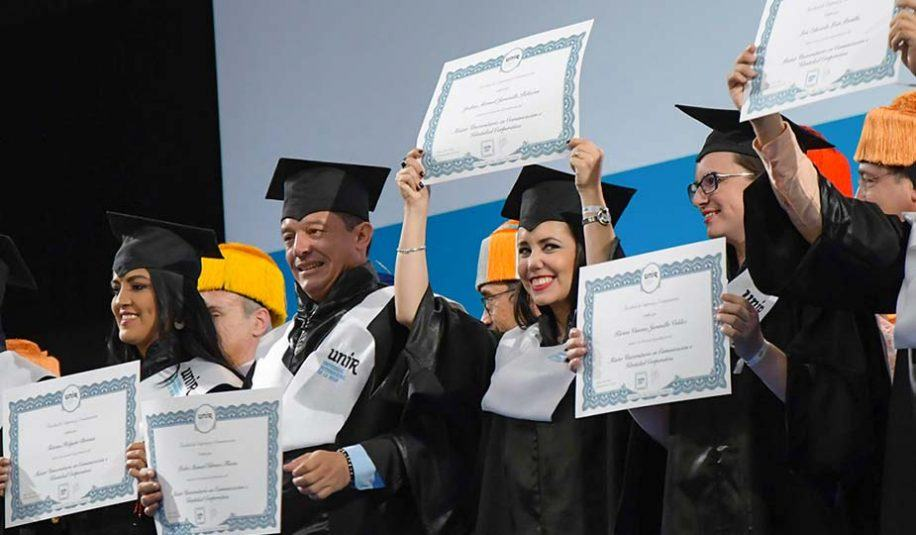
\includegraphics[width=0.7\linewidth]{Images/graduacion}
    \end{center}	
\end{frame}


\begin{frame}[fragile]{Capacitación proactiva}
    \begin{center}
        
\includegraphics[width=0.6\linewidth]{Images/sistemas}
    \end{center}	
\end{frame}

\begin{frame}[fragile]{Capacitación reactiva}
    \begin{center}
        
\includegraphics[width=0.6\linewidth]{Images/onda}
    \end{center}	
\end{frame}


\begin{frame}[fragile]{Capacitación - Formas}
   \begin{exampleblock}{Capacitación en tiempos de crisis}
    Definiremos entonces una capacitación en tiempos de crisis como una capacitación donde la inmediatez es el factor marcante.
   \end{exampleblock}

*La respuesta en una crisis como la actual suele ser e-learning pero no todos los e-learning son iguales.
\end{frame}

\begin{frame}[fragile]{Capacitación - Contenido}
\LARGE ¿Porqué la gente sigue pagando cursos, universidades y escuelas si todo se encuentra gratis en Internet?
\end{frame}

\begin{frame}[fragile]{Capacitación - Contenido}
    \LARGE Compromiso del estudiante
\end{frame}


\begin{frame}[fragile]{Capacitación - Contenido}
    \LARGE Me sobra dinero
\end{frame}

\begin{frame}[fragile]{Capacitación - Contenido}
    \LARGE Calidad del contenido
\end{frame}

\begin{frame}[fragile]{Capacitación - Contenido}
    Elementos de un modelo de e-learning (MORENO, F., BAILLY-BAILLIÈRE, M. (2002)
    \begin{itemize}
        \item Cómo: El modo de impartir la capacitación
        \item Qué: Cual sera el contenido
        \item Para qué: Objetivos y la dirección del entrenamiento
        \item Por qué: Razones puntuales de la enseñanza
        \item Cuando: Secuencia y temporalidad de los recursos
        \item Quienes: Intervienen en los recursos (creación y distribución) 
    \end{itemize}
\end{frame}

\begin{frame}[fragile]{Recomendaciones}
    \begin{itemize}
        \item Ni todo curso gratis es malo, ni todo curso pagado es bueno
        \item ¿Quien es el profesor?
        \item Evaluar clases gratuitas y demostraciones
        \item Aprender solo cosas que me parezcan interesantes/divertidas
        \item Aprender cosas "útiles"
    \end{itemize}
\end{frame}

\begin{frame}[fragile]{Capacitación - Tipos}
    Modalidad
    \begin{itemize}
        \item Clases virtuales
        \item Self paced
        \item 100\% Virtual
        \item Híbrido
    \end{itemize}

    Metodología
\begin{itemize}
    \item Centrado en tecnología (LMS)
    \item Centrado en profesor (Videoconferencias / Videos)
    \item Centrado en contenido (Self-paced)
    \item Centrado en el estudiante (Moderación en línea)
\end{itemize}
\end{frame}


\begin{frame}{Factores de éxito}
    \begin{center}
        \begin{tikzpicture}[scale=0.6, transform shape]
        \path[mindmap,concept color=blue,text=white,
        level 1 concept/.append style=
        {every child/.style={concept color=blue!70},sibling angle=-30}]
        node[concept] {E-learning}
        [clockwise from=0]
        child[concept color=blue] { node[concept] {Asesoria}}
        child[concept color=orange] { node[concept] {Evaluación}}
        child[concept color=red] { node[concept] {Comunicación sincrona o asincrona} }
        child[concept color=blue] { node[concept] {Interacción} }
        child[concept color=orange] { node[concept] {Didáctica y pédagogica} }
        child[concept color=red] { node[concept] {Calidad del contenido} }
        child[concept color=blue] { node[concept] {Material autodidacta} };
        \end{tikzpicture}
    \end{center}
\end{frame}

\begin{frame}{Factores de éxito}

        \begin{center}
            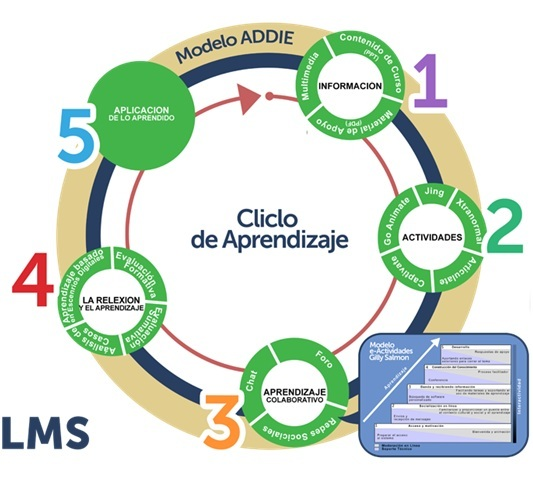
\includegraphics[width=0.4\linewidth]{Images/modelogalileo}
        \end{center}

        Fuente: Miguel Morales - http://www.galileo.edu/ivn/noticias/caracteristicas-de-un-modelo-efectivo-de-elearning/

\end{frame}

\begin{frame}[fragile]{VideoConferencias}
    
Video con interacción
    \begin{itemize}
    \item Youtube on air
    \item Facebook Live
    \item Crowdcast
\end{itemize}

Video sin interacción
\begin{itemize}
    \item Canales de Youtube
    \item Canales de Twitch
\end{itemize}

\end{frame}

\begin{frame}[fragile]{Self-paced}
    
    \begin{itemize}
        \item Udemy
        \item Khan Academy
        \item Pathwright
        \item Teachable
        \item CourseSites
    \end{itemize}
    
\end{frame}


\begin{frame}{Víctor Orozco}
\begin{columns}[T] % contents are top vertically aligned
	
	\begin{column}[T]{4cm} % alternative top-align that's better for graphics
		\begin{figure}
			\centering
			
\includegraphics[width=\linewidth]{Images/logos}
		\end{figure}
	\end{column}
	\begin{column}[T]{6cm} % each column can also be its own environment
		\begin{itemize}
			\item vorozco@nabenik.com
			\item \href{https://twitter.com/tuxtor}{@tuxtor}
			\item \href{http://vorozco.com}{http://vorozco.com}
			\item \href{http://tuxtor.shekalug.org}{http://tuxtor.shekalug.org} 
		\end{itemize}
		\begin{center}
			
\includegraphics[width=0.1\linewidth]{Images/cclogo}
			\\
			This work is licensed under Creative Commons Attribution-NonCommercial-ShareAlike 3.0 Guatemala (CC BY-NC-SA 3.0 GT).
		\end{center}
	\end{column}
\end{columns}
\end{frame}

{
    \usebackgroundtemplate{
\includegraphics[width=\paperwidth]{Images/final}}
\begin{frame}
\end{frame}
}

\end{document}

